\textbf{5-1.}光滑水平面上并排静放着两块质量分别为 $m_{1}$ 和 $m_{2}$ 的木块。一质量为 $m$ 的子弹以 $v_{0}$ 的初速度水平地射向两木块，若 $m_{1} = 2m_{0}, m_{2} = m_{0}$ ，质量为 $m$ 的子弹水平射穿 $m_{1}$ 后，射入 $m_{2}$ 内。当子弹相对 $m_{2}$ 静止时， $m_{2}$ 的速度是 $m_{1}$ 的两倍。求此过程中摩擦阻力所做的功。

\vfill

\textbf{5-2.}汽车沿着一坡度不大的斜坡以 $v_{1} = 12 \mathrm{~m} / \mathrm{s}$ 的速率向上匀速行驶, 当此车用同样的功率沿斜坡向下匀速行驶时, 车速为 $v_{2} = 20 \mathrm{~m} / \mathrm{s}$ 。若此车保持功率不变而沿同样的水平路面以匀速 $v$ 行驶, 设汽车在水平路面上受到的阻力与在斜坡上受到的阻力相同, 求 $v$ 的大小。

\vfill
\newpage

\textbf{5-3.}一质点在保守力场中沿 $x$ 轴（在 $x > 0$ 范围内）运动，其势能为 $E_{\mathrm{p}} = \frac{kx}{x^{2} + a^{2}}$ 。式中 $k, a$ 均为大于零的常量。试求：

(1) 质点所受到的力的表示式;

(2) 质点的平衡位置；

(3) 若质点静止在平衡位置,试讨论平衡的稳定性。

\vfill

\textbf{5-4.}一块长为 $l$ , 质量为 $m_{0}$ 的木板静置于光滑的水平桌面上, 在板的左端有一质量为 $m$ 的小物体 (大小可忽略) 以 $v_{0}$ 的初速度相对板向右滑动, 当它滑至板的右端时相对板静止。试求:

(1) 物体与板之间的摩擦因数;

(2) 在此过程中板的位移。

\vfill
\newpage

\textbf{5-5.}在倾角为 $\theta$ 的斜面上, 一质量为 $m$ 的物体通过一劲度系数为 $k$ 的弹簧与固定在斜面上的挡板相连, 如习题 5- 5 图所示。物体与斜面间的摩擦因数为

$\mu$ 。开始时，m 静止，弹簧处于原长。现有一沿斜面向上的恒力 F 作用在 m 上，使 m 沿斜面向上滑动。试求：从 m 开始运动到它运动到最高位置过程中力 F 所做的功。

\begin{figure}[H]
  \centering
  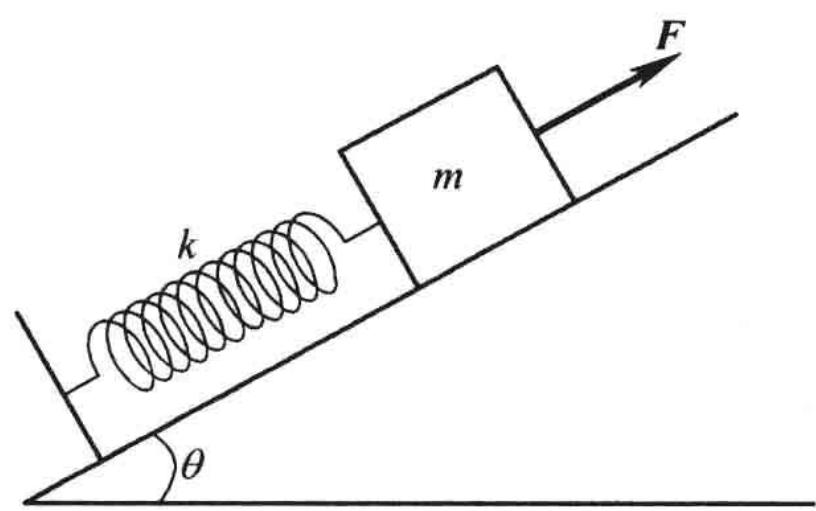
\includegraphics[width=0.3\textwidth]{figures/fig5-5.jpg}
  \end{figure}

\vfill

\textbf{5-6.}一小球做竖直上抛运动, 当它回到抛出点时, 速度为抛出时的 $3 / 4$ 。设小球运动中受到的空气阻力为恒力。试求:

(1) 小球受到的空气阻力与重力之比;

(2) 小球上升的最大高度与真空情况下最大高度之比 $(g = 10 \mathrm{~m} / \mathrm{s}^{2})$ 。

\vfill
\newpage

\textbf{5-7.}如习题 5-7 图所示, 质量为 $m$ 的物体以 $v_{0}$ 的速度在光滑水平面上沿 $x$ 轴正方向运动, 当它到达原点 $O$ 时, 撞击一劲度系数为 $k$ 的轻弹簧, 并开始受到摩擦力的作用,摩擦因数是位置的函数,可表示为 $\mu = ax$ (a 为一较小的常量)。求物体第一次返回 O 点时的速度。

\begin{figure}[H]
  \centering
  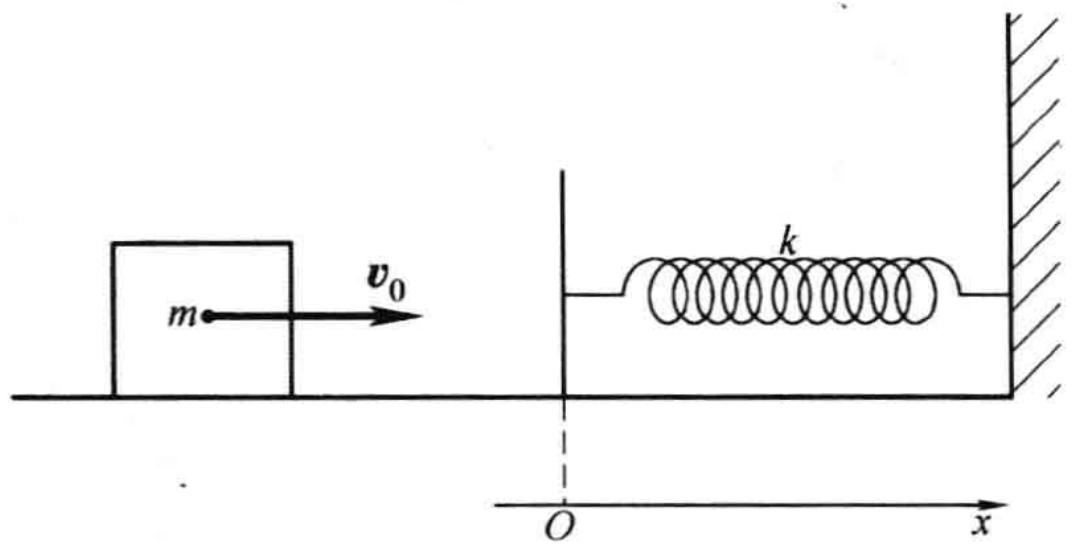
\includegraphics[width=0.35\textwidth]{figures/fig5-7.jpg}
  \end{figure}

\vfill

\textbf{5-8.}质量为 $m$ 的小球通过一根长为 $2l$ 的细绳悬挂于 $O$ 点。在 $O$ 点的正

下方 l 远处有一个固定的钉子 P。开始时，把绳拉至水平位置，然后释放小球。试求：当细绳碰到钉子后小球所能上升的最大高度。

\begin{figure}[H]
  \centering
  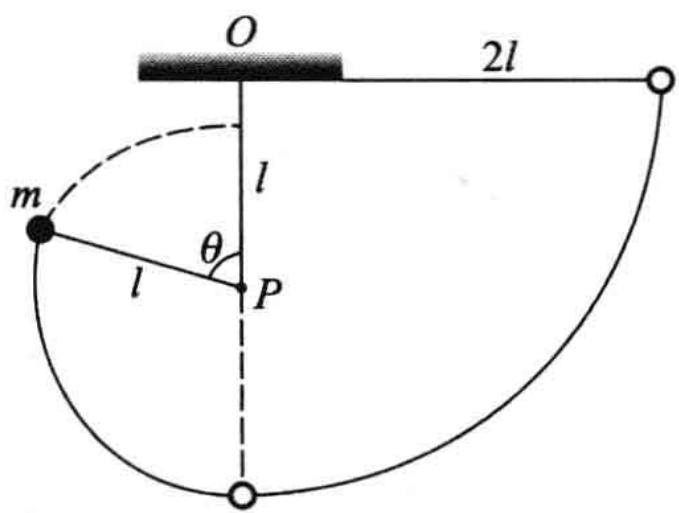
\includegraphics[width=0.25\textwidth]{figures/fig5-8.jpg}
  \end{figure}

\vfill
\newpage

\textbf{5-9.}如习题 5-9 图所示, 质量为 $m_{0}$ 的两质点分别固定在 $x$ 轴上的 $A(-a, 0)$ 、 $B(a,0)$ 两点, 若有一质点 $m$ 在万有引力作用下从 $y=3a$ 处由静止开始向原点运动。试求质点经过原点时的速度。

\begin{figure}[H]
  \centering
  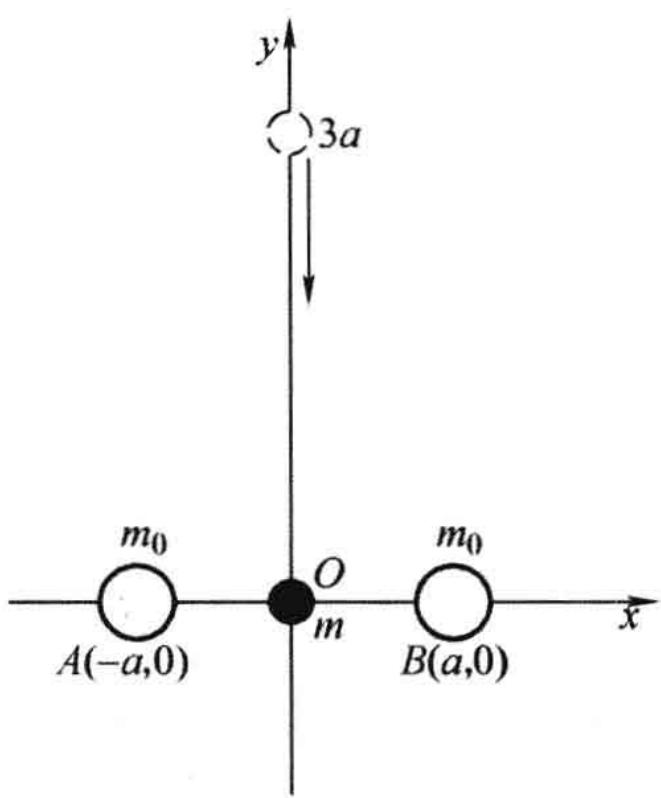
\includegraphics[width=0.25\textwidth]{figures/fig5-9_5.jpg}
  \end{figure}

\vfill

\textbf{5-10.}某人在地面上双脚起跳可使他的重心升高 $h$ 。现在他和另一个体重同为 $m_{1}$ 的人分别站在轻滑轮两边的秤盘中，如习题5-10图所示。盘重均为

$m_{2}$ 。试求:当此人在秤盘中用和在地面上起跳同样的能量双脚起跳时,他的重心可升高多少?

\begin{figure}[H]
  \centering
  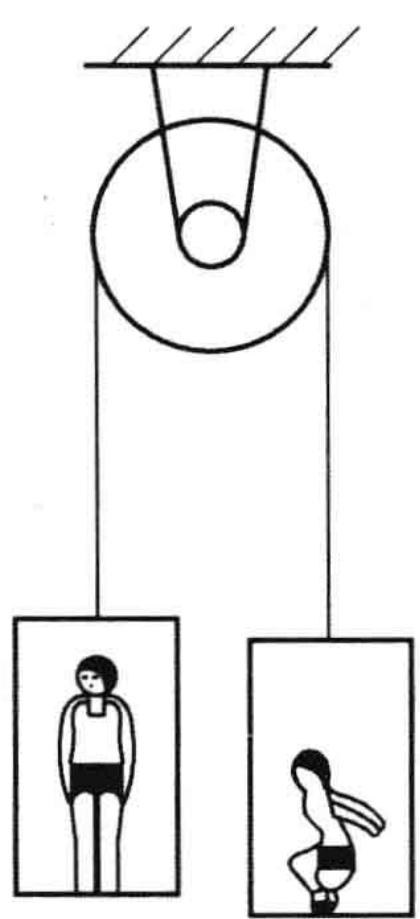
\includegraphics[width=0.13\textwidth]{figures/fig5-10.jpg}
  \end{figure}

\vfill
\newpage

\textbf{5-11.}在光滑半球形碗底静放着一质量 $m = 50 \mathrm{~g}$ 的光滑小球 B, 另一与 B 完全相同的小球 A 从高为 $h = 5.0 \mathrm{~cm}$ 的碗内壁处由静止滑下。若 A、B 球的碰撞为非弹性碰撞, 恢复系数为 $e = 0.6$ 。求 B 球被碰后能升多高?

\vfill

\textbf{5-12.}在光滑的水平桌面上有三个弹性小环 A、B、C, 它们的质量分别为 $m$ 、 $m 、 \alpha m (\alpha > 1)$ , 并依次排列在一条直线上。开始时, B、C 静止, 并挨在一起, 而 A 以 $v_{0}$ 的速度向 B 运动。试证明, 当它们之间的碰撞结束时, B 环静止, 而 A、C 的运动状态和没有 B 环时 A、C 碰撞后的运动状态一样。

\vfill
\newpage


\textbf{5-13.}一小球与两个相同的弹簧相连, 如习题 5-13 图所示。当小球平衡时, 两弹簧均受到拉伸。若忽略重力, 试讨论小球平衡的稳定性。

\begin{figure}[H]
  \centering
  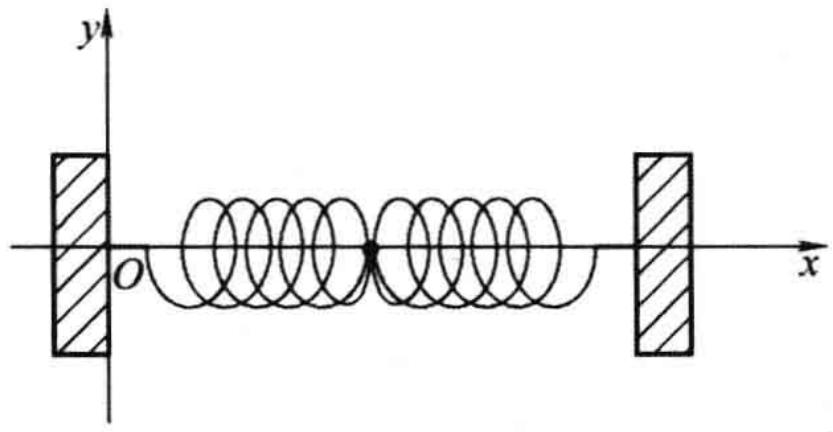
\includegraphics[width=0.35\textwidth]{figures/fig5-13.jpg}
  \end{figure}

\vfill

\textbf{5-14.}一质量为 $m$ 的质点在保守力的作用下沿 $x$ 轴（在 $x > 0$ 范围内）运动，其势能的数值为： $E_{\mathrm{p}} = \frac{A}{x^3} - \frac{B}{x}$ ，其中 $A, B$ 均为大于零的常量。

(1) 画出势能曲线图；

(2) 确定势阱的深度(最低点势能值);

（3）找出质点运动中受到沿 x 轴负方向最大力的位置；

(4) 若质点的总能量 E=0，试确定质点的运动范围。（本题中 x 以 m 为单位， $E_{p}$ 以 J 为单位。）

\begin{figure}[H]
  \centering
  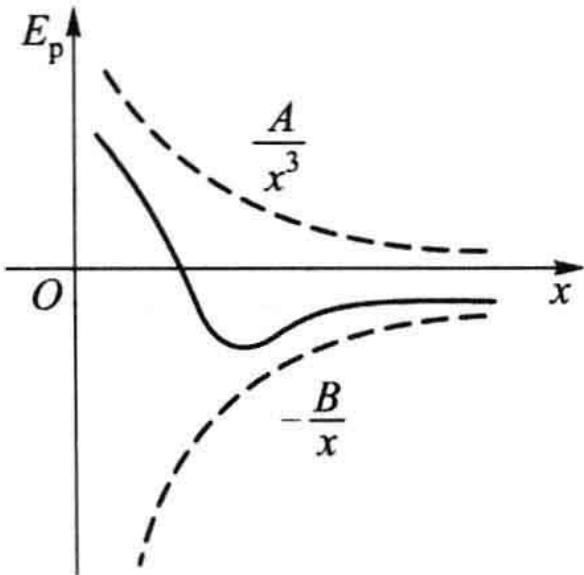
\includegraphics[width=0.25\textwidth]{figures/fig5-14_2.jpg}
  \end{figure}

\vfill
\newpage

\textbf{5-15.}一质量为 $m$ 的质点在保守力的作用下沿 $x$ 轴方向运动, 其势能的数值为: $E_{\mathrm{p}} = ax^{2}(b - x)(x$ 的单位是 $\mathrm{m}, E_{\mathrm{p}}$ 的单位是 $\mathrm{J}$ ), 其中 $a, b$ 均为大于零的常量。

(1) 试求质点所受力的表达式;

(2) 画出势能曲线图；

(3) 确定平衡位置,并讨论平衡位置的稳定性;

(4) 若质点从原点 $x = 0$ 处以 $v_{0}$ 开始运动, 试问, $v_{0}$ 在什么范围内质点不可能到达无穷远?

\begin{figure}[H]
  \centering
  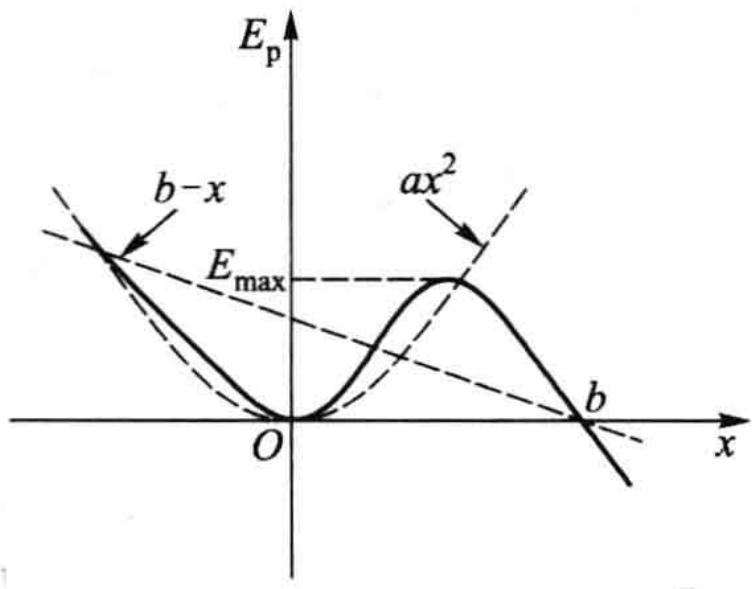
\includegraphics[width=0.3\textwidth]{figures/fig5-15.jpg}
  \end{figure}

\vfill

\textbf{5-16.}一颗质量为 $m$ 的人造地球卫星以圆形轨道环绕地球飞行。由于受到空气阻力的作用, 其轨道半径从 $r_1$ 变小到 $r_2$ 。求在此过程中空气阻力所做的功。

\vfill
\newpage

\textbf{5-17.}如习题 5-17 图所示, 物体从高为 $h$ 的斜面顶端自静止开始滑下, 最后停在与起点的水平距离为 $s$ 的水平地面上。若物体与斜面和与地面间的摩擦因数均为 $\mu$ , 证明 $\mu = h / s$ 。

\begin{figure}[H]
  \centering
  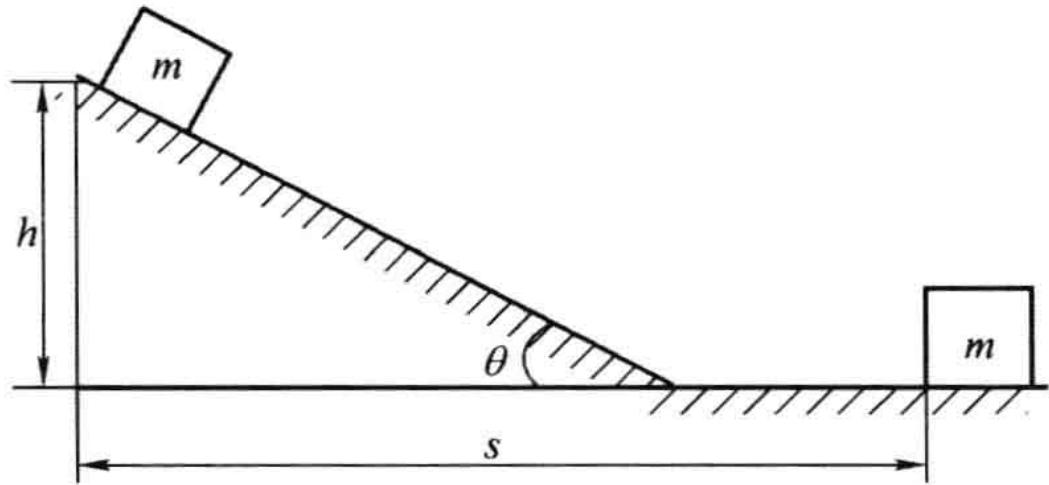
\includegraphics[width=0.35\textwidth]{figures/fig5-17.jpg}
  \end{figure}

\vfill

\textbf{5-18.}若上题中物体与斜面间摩擦因数和物体与地面之间的摩擦因数并不相同。当物体自斜面顶端静止滑下时, 停在地面上的 $A$ 点, 而当物体以 $v_{0}$ 的初速度 (方向沿斜面向下) 自同一点滑下时, 则停在地面上的 $B$ 点。已知 $A 、 B$ 点与斜面底端 $C$ 点的距离之间满足 $B C = 2 A C$ 。试求物体在斜面上运动的过程中摩擦力所做的功。

\vfill
\newpage

\textbf{5-19.}一光滑圆环, 半径为 $R$ , 用细线悬挂在支点上。环上穿有质量都是 $m$ 的两颗珠子, 让两珠子从环顶同时静止释放并向两边下滑。若圆环的质量为 $m_0$ , 试证明: 只有当 $m > \frac{3}{2} m_0$ 时, 圆环才会升起, 并求出珠子所在半径与细线所在竖直线的夹角 $\theta$ 。

\begin{figure}[H]
  \centering
  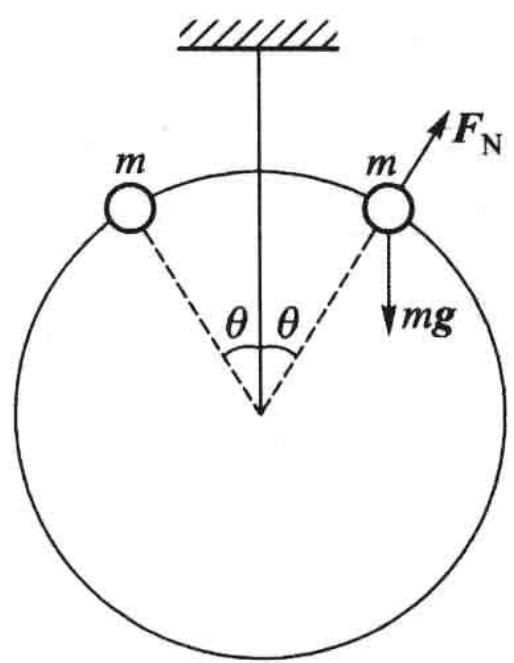
\includegraphics[width=0.23\textwidth]{figures/fig5-19.jpg}
  \end{figure}

\vfill

\textbf{5-20.}物体沿习题 5-20 图所示的光滑轨道自点 $A$ 由静止开始滑下。轨道的圆环部分有一对称的缺口 $BC$ , 缺口的张角 $\angle BOC = 2\alpha$ , 圆环的半径为 $R$ 。试问: A 点的高度 h 应等于多少才能使物体恰好越过缺口而走完整个圆环?

\begin{figure}[H]
  \centering
  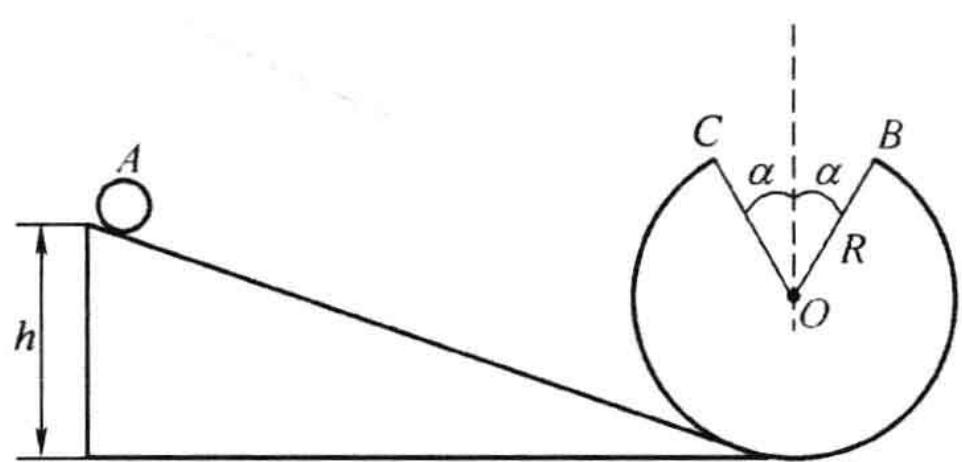
\includegraphics[width=0.35\textwidth]{figures/fig5-20.jpg}
  \end{figure}

\vfill
\newpage

\textbf{5-21.}如习题 5-21 图所示, 质量为 $m$ 的物体从光滑轨道的顶端 $A$ 点, 由静止开始沿斜道滑下, 在半径为 $R$ 的圆环部分的最低点 $B$ 与另一质量为 $m_0$ 的静止物体发生弹性碰撞, 碰后 $m_0$ 沿圆环上升, 并在高度为 $h_0$ 处脱离圆环, 而 $m$ 则沿斜道上升后又滑下, 并在 $m_0$ 脱离点脱离圆环。试求:

(1) m 与 $m_{0}$ 之比；

(2) A 点的高度 h。

\begin{figure}[H]
  \centering
  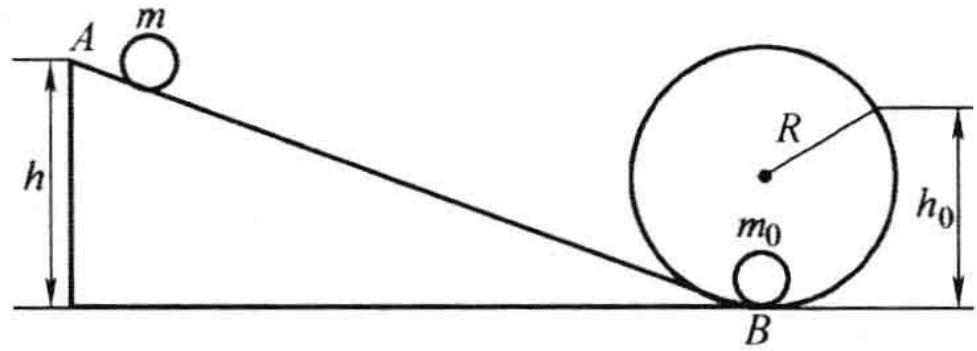
\includegraphics[width=0.32\textwidth]{figures/fig5-21.jpg}
  \end{figure}

\vfill

\textbf{5-22.}质量分别为 $m_{1}$ 和 $m_{2}$ 的两个物块由一劲度系数为 $k$ 的轻弹簧相连, 竖直地放在水平桌面上, 如习题 5-22 图所示。另有一质量为 $m$ 的物体从高出 $m_{1}$ 为 $h$ 的地方由静止开始自由落下, 当与 $m_{1}$ 发生碰撞后, 即与 $m_{1}$ 黏合在一起向下运动。试问 $h$ 至少应多大, 才能使得弹簧反弹后 $m_{2}$ 与桌面互相脱离?

\begin{figure}[H]
  \centering
  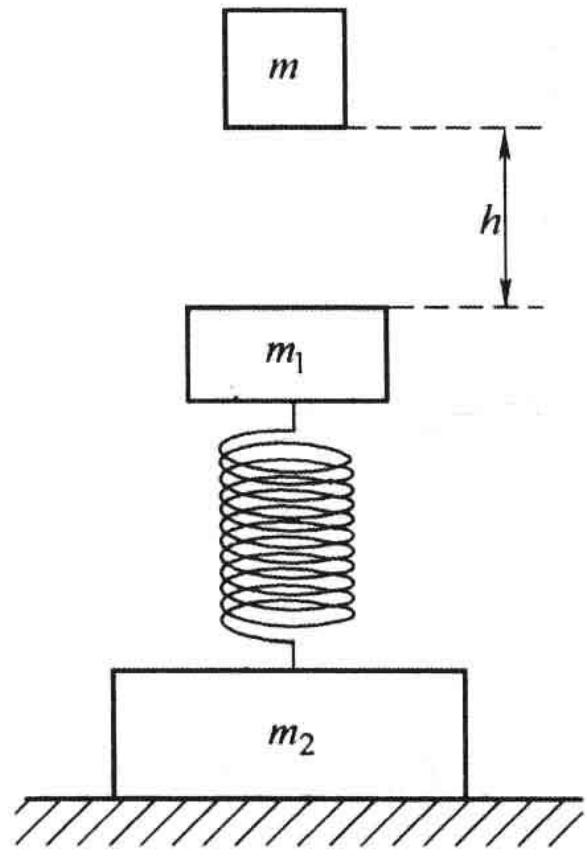
\includegraphics[width=0.2\textwidth]{figures/fig5-22.jpg}
  \end{figure}

\vfill
\newpage

\textbf{5-23.}在水平桌面上, 质量分别为 $m_{1}$ 和 $m_{2}$ 的两物块由一劲度系数为 $k$ 的弹簧相连。物块与桌面间的摩擦因数均为 $\mu$ 。开始时, 弹簧处于原长, $m_{2}$ 静止, 而 $m_{1}$ 以 $v_{0} = \sqrt{\frac{6m_{1}m_{2}g^{2}\mu^{2}}{k(m_{1} + m_{2})}}$ 的速度拉伸弹簧。试求: 当弹簧达最大拉伸时的伸长量 (设 $m_{1} > m_{2}$ ) 。

\vfill

\textbf{5-24.}质量分别为 $m_{1}$ 和 $m_{2}$ 的两物体发生非弹性正碰, 恢复系数为 $e$ 。试证明: 在质心坐标系中碰撞时损失的动能为其初始动能的 $(1 - e^{2})$ 倍。

\vfill
\newpage

\textbf{5-25.}长为 $2a$ 的轻绳两端各系有一质量为 $m$ 的小球, 中点处系有一质量为 $m_0$ 的小球, 三球排成一直线静置于光滑水平台面, 绳恰被拉直。对小球 $m_0$ 施以冲力, 使其获得与绳垂直的初速度 $v_0$ , 求:

(1) 当两小球 m 相碰的瞬时各球的速率;

(2) 当两小球 m 相碰的瞬时绳中的张力;

(3) 若从 $m_0$ 启动到两球 $m$ 相碰历时 $t$ , 而在此期间 $m_0$ 行进的距离为 $x$ , 试证明: $(m_0 + 2m)x = m_0v_0t + 2ma$ 。

\vfill

\textbf{5-26.}边长为 $a$ 的正方体木块静浮于横截面积为 $4a^{2}$ 的杯内水面上, 水的深

度 $h = 2a$ 。已知水的密度为 $\rho_0$ ，木块的密度为 $\frac{1}{2}\rho_0$ ，现将木块非常缓慢地压至水底。忽略水的阻力作用，求在此过程中外力所做的功。

\begin{figure}[H]
  \centering
  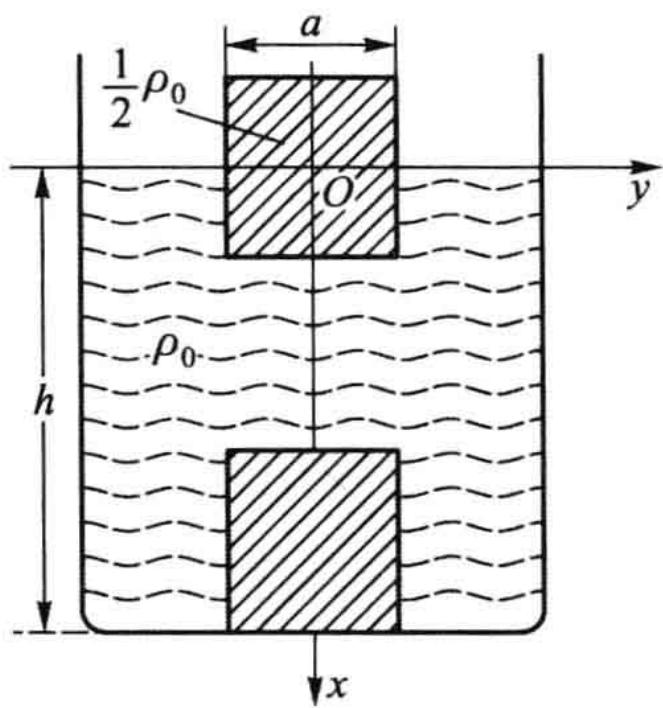
\includegraphics[width=0.25\textwidth]{figures/fig5-26.jpg}
  \end{figure}

\vfill
\newpage

\textbf{5-27.}一条长为 $2 l$ 、质量为 $m$ 的柔软绳索, 挂在一光滑的水平轴钉 (粗细可忽略) 上, 当两边的绳长均为 $l$ 时, 绳索处于平衡状态。若给其一端加一个竖直方向的微小扰动, 则绳索就从轴钉上滑落。试求:

(1) 当绳索刚脱离轴钉时, 绳索的速度;

(2) 当较长的一边绳索的长度为 x 时, 轴钉上所受的力。

\vfill

\textbf{5-28.}在竖直平面内有一光滑的半圆形管道, 圆的半径为 $R$ 。管内有一条

长度正好为半圆周长 $\pi R$ 的链条, 其线密度为 $\rho_{l}$ , 如习题 5-28 图所示。若由于微小的扰动, 链条从管口向外滑出。试求:

（1）当链条刚从管口全部滑出时的速度；

(2) 当链条从管口滑出的长度为 $\frac{\pi}{3} R$ 时的速度和加速度。

\begin{figure}[H]
  \centering
  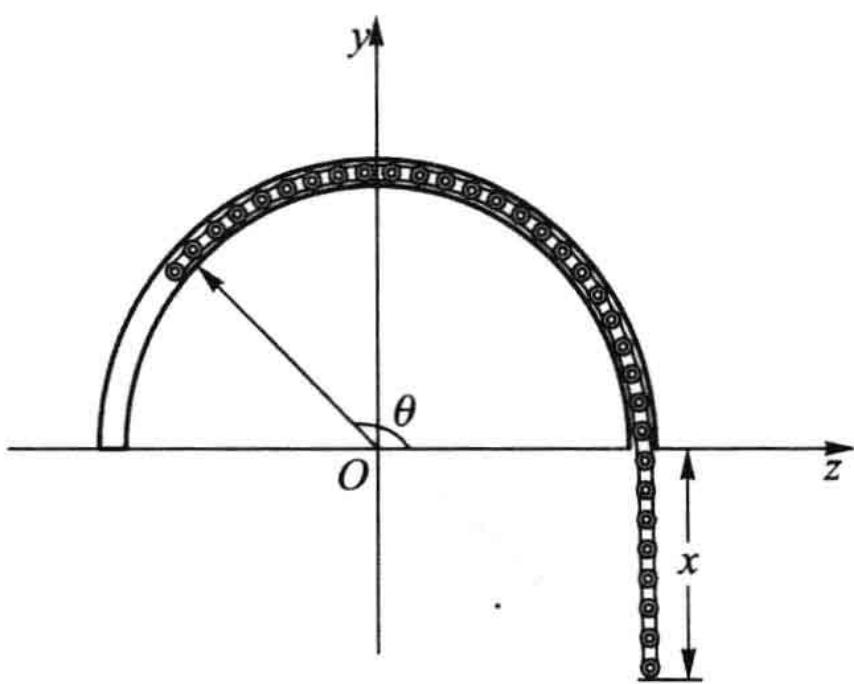
\includegraphics[width=0.33\textwidth]{figures/fig5-28.jpg}
  \end{figure}

\vfill
\newpage

\textbf{5-29.}在倾角 $\theta = \arctan \frac{3}{4}$ 的光滑斜面上叠放着质量 $m_{1} = 40 \mathrm{~kg}$ 的重物和质量 $m_{2} = 20 \mathrm{~kg}$ 、长 $l = 0.2 \mathrm{~m}$ 的板, 重物与板之间的摩擦因数 $\mu = 0.5$ 。 $m_{1}$ 与另一质量 $m = 30 \mathrm{~kg}$ 的重物由一跨过装在斜面顶端的定滑轮的细绳相连, 如习题 5-29 图所示。开始时, $m_{1}$ 和 $m_{2}$ 均静靠在斜面上一挡板处, $m$ 由手托住, 使绳松弛, 然后放手, 当 $m$ 自由下落的高度为 $h$ 时, 绳被拉紧。若 $m_{1}$ 体积很小, 以致可忽略其线度, 并设斜面和 $m$ 的运动长度足够长。忽略绳与滑轮的质量和滑轮轴承处的摩擦力。

（1）试分析由此三物体组成的系统以后运动的情况；

(2) 一种分析是, 若 $h$ 不太大时, 则 $m_{1}$ 和 $m_{2}$ 在以后的运动过程中不会互相脱离。这种分析是否正确? 如是正确的话, 求出 $h$ 的最大值。

\begin{figure}[H]
  \centering
  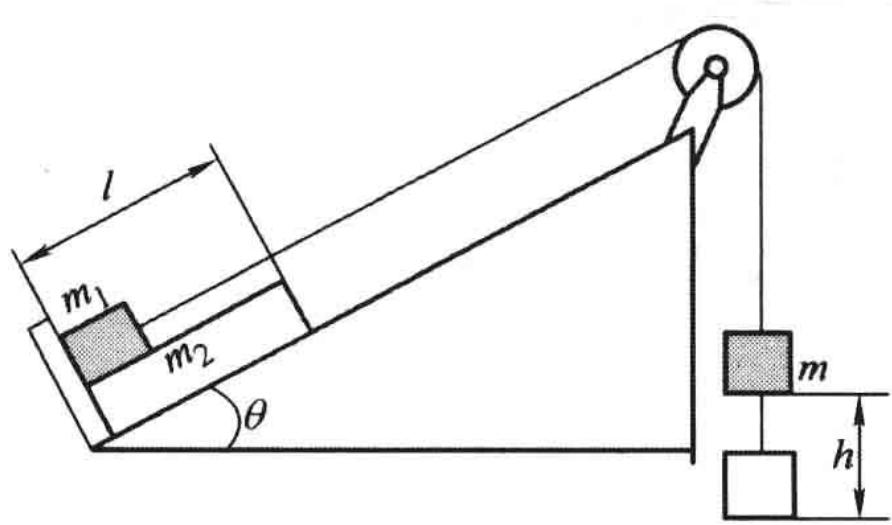
\includegraphics[width=0.3\textwidth]{figures/fig5-29.jpg}
  \end{figure}

\vfill

\textbf{5-30.}如习题 5-30 图所示,一个人手持质量为 $m$ 的小球乘坐在热气球下的吊篮里。气球、吊篮和人的总质量为 $m_0$ 。整个系统静止在空中。突然,人将小球向上急速抛出,经过时间 $t$ 后小球又返回人手中。若人手在抛接球时相对吊篮的位置不变,试求人在抛球过程中对系统做的功。

\begin{figure}[H]
  \centering
  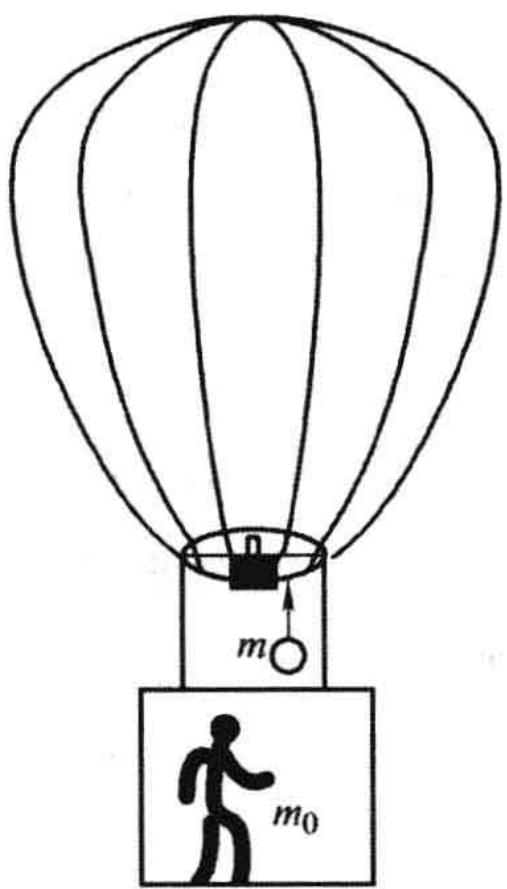
\includegraphics[width=0.2\textwidth]{figures/fig5-30.jpg}
  \end{figure}

\vfill
\newpage

\textbf{5-31.}在光滑的水平面上有两个质量分别为 $m_{1}$ 和 $m_{2} (m_{1} < m_{2})$ 的物块, $m_{2}$ 上连有一轻弹簧, 如习题 5-31 图所示。第一次, 具有动能 $E_{0}$ 的 $m_{1}$ 与静止的 $m_{2}$ 相碰; 第二次, 具有动能 $E_{0}$ 的 $m_{2}$ 与静止的 $m_{1}$ 相碰, 两次碰撞均压缩轻弹簧。试问:

(1) 两次碰撞中哪一次弹簧的最大压缩量较大?

(2) 若碰前两物块的总动能为 $E_{0}$ , 则 $E_{0}$ 如何分配, 才能使在两物块碰撞过程中弹簧的最大压缩量最大?

\begin{figure}[H]
  \centering
  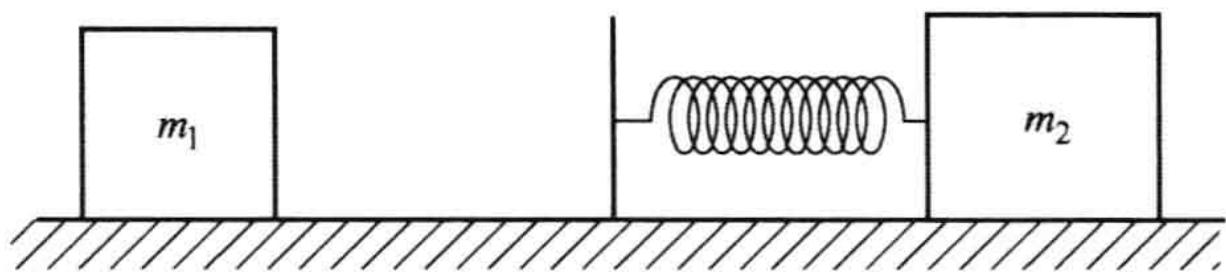
\includegraphics[width=0.35\textwidth]{figures/fig5-31_1.jpg}
  \end{figure}

\vfill

\textbf{5-32.}在光滑的水平面上, 一质量为 $m_{0}$ 的架子内连有一劲度系数为 $k$ 的弹簧,如习题5-32图所示。一质量为 $m$ 的小球以 $\pmb{u}$ 的速度射入静止的架子内,并开始压缩弹簧。设小球与架子内壁间无摩擦力。试求:

(1) 弹簧的最大压缩量；

(2) 从弹簧被压缩到弹簧达最大压缩量所需的时间；

(3) 在此过程中架子的位移。

\begin{figure}[H]
  \centering
  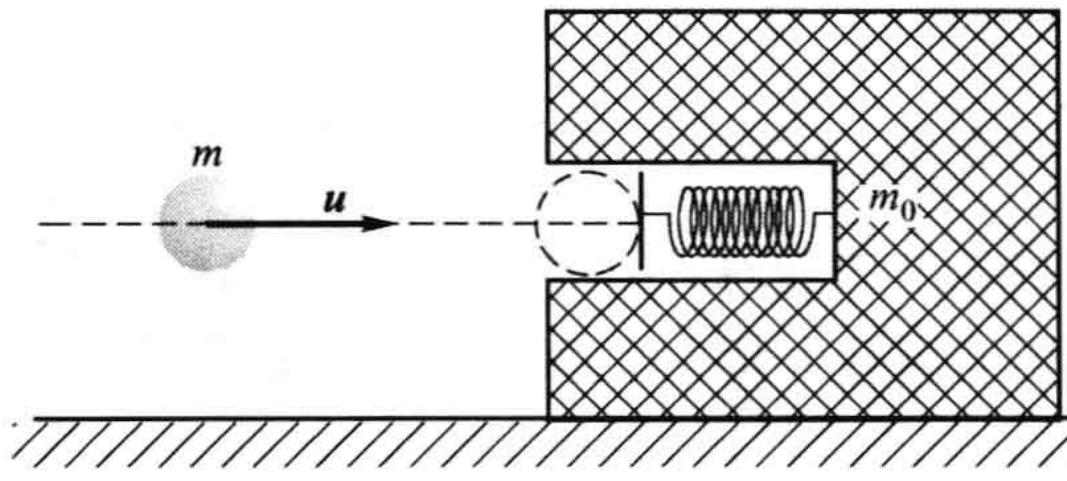
\includegraphics[width=0.33\textwidth]{figures/fig5-32.jpg}
  \end{figure}

\vfill
\newpage

\textbf{5-33.}在光滑的水平桌面上有三个完全相同光滑弹性小球, 两个静止小球 B、C 互相紧靠着, 另一小球 A 则以 $v_{0}$ 的速度沿 B、C 球心连线的中垂线向着两球运动。求碰后三球的速度。

\vfill

\textbf{5-34.}一运动粒子与另一质量与其相等的静止粒子发生弹性斜碰,试证

明:碰撞后两粒子的运动方向彼此垂直。

\begin{figure}[H]
  \centering
  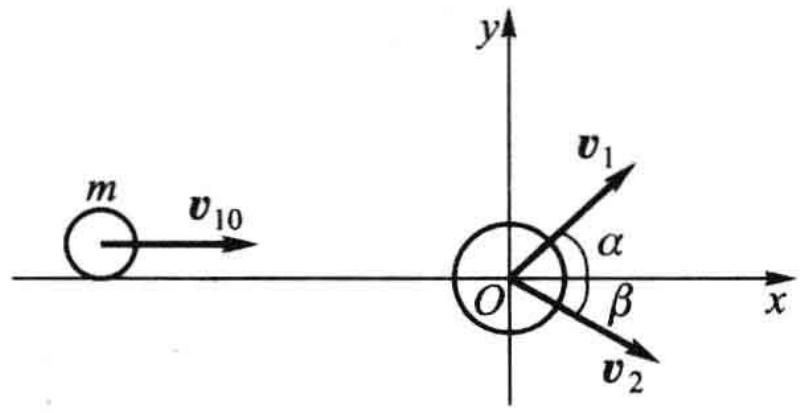
\includegraphics[width=0.4\textwidth]{figures/fig5-34.jpg}
  \end{figure}

\vfill
\newpage

\textbf{5-35.}一质量为 $2 \mathrm{~kg}$ 的小球 A 以 $v_{\mathrm{A} 0} = 32 \mathrm{~m} / \mathrm{s}$ 的速度与另一质量为 $6 \mathrm{~kg}$ 的静止小球 B 相碰。设碰撞是弹性的, 则在质心坐标系中, 两小球的反射角均为 $90^{\circ}$ 。试问:

(1) 在实验室坐标系中, A 球的反射角为多大?

(2) 在实验室坐标系中, 碰后 B 球的运动方向与 A 球原运动方向之间的夹角为多大?

\begin{figure}[H]
  \centering
  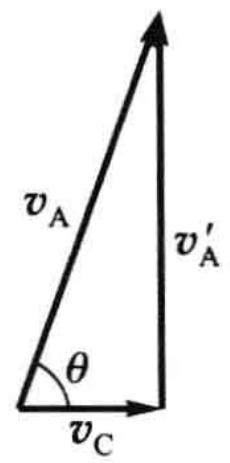
\includegraphics[width=0.1\textwidth]{figures/fig5-35_b.jpg}
  \end{figure}

\vfill

\textbf{5-36.}一质量为 $m$ 的质子以 $v_{0}$ 的速度去撞击静止质量为 $4 m$ 的氦核。在实验室坐标系里, 质子以 $\frac{1}{2} v_{0}$ 的速度和 $30^{\circ}$ 角散射。试求:

(1) 在实验室坐标系里, 撞击后氦核的速度及运动方向;

(2) 在质心坐标系里质子的散射速度, 以及两粒子的散射角度;

(3) 系统在散射中总能量的变化。

\vfill
\newpage
